\documentclass[]{article}
\usepackage{lmodern}
\usepackage{amssymb,amsmath}
\usepackage{ifxetex,ifluatex}
\usepackage{fixltx2e} % provides \textsubscript
\ifnum 0\ifxetex 1\fi\ifluatex 1\fi=0 % if pdftex
  \usepackage[T1]{fontenc}
  \usepackage[utf8]{inputenc}
\else % if luatex or xelatex
  \ifxetex
    \usepackage{mathspec}
  \else
    \usepackage{fontspec}
  \fi
  \defaultfontfeatures{Ligatures=TeX,Scale=MatchLowercase}
\fi
% use upquote if available, for straight quotes in verbatim environments
\IfFileExists{upquote.sty}{\usepackage{upquote}}{}
% use microtype if available
\IfFileExists{microtype.sty}{%
\usepackage{microtype}
\UseMicrotypeSet[protrusion]{basicmath} % disable protrusion for tt fonts
}{}
\usepackage[margin=1in]{geometry}
\usepackage{hyperref}
\hypersetup{unicode=true,
            pdfborder={0 0 0},
            breaklinks=true}
\urlstyle{same}  % don't use monospace font for urls
\usepackage{longtable,booktabs}
\usepackage{graphicx,grffile}
\makeatletter
\def\maxwidth{\ifdim\Gin@nat@width>\linewidth\linewidth\else\Gin@nat@width\fi}
\def\maxheight{\ifdim\Gin@nat@height>\textheight\textheight\else\Gin@nat@height\fi}
\makeatother
% Scale images if necessary, so that they will not overflow the page
% margins by default, and it is still possible to overwrite the defaults
% using explicit options in \includegraphics[width, height, ...]{}
\setkeys{Gin}{width=\maxwidth,height=\maxheight,keepaspectratio}
\IfFileExists{parskip.sty}{%
\usepackage{parskip}
}{% else
\setlength{\parindent}{0pt}
\setlength{\parskip}{6pt plus 2pt minus 1pt}
}
\setlength{\emergencystretch}{3em}  % prevent overfull lines
\providecommand{\tightlist}{%
  \setlength{\itemsep}{0pt}\setlength{\parskip}{0pt}}
\setcounter{secnumdepth}{5}
% Redefines (sub)paragraphs to behave more like sections
\ifx\paragraph\undefined\else
\let\oldparagraph\paragraph
\renewcommand{\paragraph}[1]{\oldparagraph{#1}\mbox{}}
\fi
\ifx\subparagraph\undefined\else
\let\oldsubparagraph\subparagraph
\renewcommand{\subparagraph}[1]{\oldsubparagraph{#1}\mbox{}}
\fi

%%% Use protect on footnotes to avoid problems with footnotes in titles
\let\rmarkdownfootnote\footnote%
\def\footnote{\protect\rmarkdownfootnote}

%%% Change title format to be more compact
\usepackage{titling}

% Create subtitle command for use in maketitle
\newcommand{\subtitle}[1]{
  \posttitle{
    \begin{center}\large#1\end{center}
    }
}

\setlength{\droptitle}{-2em}
  \title{}
  \pretitle{\vspace{\droptitle}}
  \posttitle{}
  \author{}
  \preauthor{}\postauthor{}
  \predate{\centering\large\emph}
  \postdate{\par}
  \date{16 March, 2018}

\usepackage{bbm} 
\newcommand{\D}{\text{d}}
\newcommand{\indicator}{\mathbbm{1}}
\newcommand{\hamm}{d_h}
\newcommand{\symhamm}{d_{sh}}
\newcommand{\hz}{\text{Hz}}
\newcommand{\tr}{\text{tr}}
\newcommand{\Iext}{{I_e/A}}
\newcommand\gvn[1][]{\:#1\vert\:}
\usepackage{afterpage}
\usepackage{fancyvrb}
\usepackage{longtable}
\usepackage{booktabs} 
\usepackage{placeins}

\usepackage{amsthm}
\newtheorem{theorem}{Theorem}[section]
\newtheorem{lemma}{Lemma}[section]
\theoremstyle{definition}
\newtheorem{definition}{Definition}[section]
\newtheorem{corollary}{Corollary}[section]
\newtheorem{proposition}{Proposition}[section]
\theoremstyle{definition}
\newtheorem{example}{Example}[section]
\theoremstyle{definition}
\newtheorem{exercise}{Exercise}[section]
\theoremstyle{remark}
\newtheorem*{remark}{Remark}
\newtheorem*{solution}{Solution}
\begin{document}

{
\setcounter{tocdepth}{2}
\tableofcontents
}
\subsection{Inferring a three variable Bayesian
network}\label{inferring-a-three-variable-bayesian-network}

I reparametrise the joint probability of the graph by replacing the
conditional probability \(P(child|parent)\) to be the quotient of two
joint distirbution \(\frac{P(child,parent)}{P(parent)}\). Because
\(P(child|parent)\) enters the marginalised likelihood as a
Beta-Binomial probability, \(P(parent)\) enters the term as a
Drichlet-Multinomial probability:

\[
P(x_k)={\frac {\left(n!\right)\Gamma \left(\sum \alpha _{k}\right)}{\Gamma \left(n+\sum \alpha _{k}\right)}}\prod _{k=1}^{K}{\frac {\Gamma (x_{k}+\alpha _{k})}{\left(x_{k}!\right)\Gamma (\alpha _{k})}}
\] where \(\sum{x_k}=N\) is the partition of sample into k categories,
\(\alpha_k\) is the imaginary sample size for each category (also known
as prior concentration). This formulation has the advantage of easier
coding.

To be consistent with bnlearn and deal, I did discared the multinomial
terms in the calculation, leading to

\[
P(x_k)={\frac {\Gamma \left(\sum \alpha _{k}\right)}{\Gamma \left(n+\sum \alpha _{k}\right)}}\prod _{k=1}^{K}{\frac {\Gamma (x_{k}+\alpha _{k})}{\Gamma (\alpha _{k})}}
\]

\subsection{Number of Bayesian
networks:}\label{number-of-bayesian-networks}

A V-variable network has \(V(V-1)/2\) bivariate interaction (edges),
each interaction can have 3 possible status (A-\textgreater{}B,
A\textless{}-B, A B). Hence altogether there are \(n(V) = 3^{V(V-1)/2}\)
possible networks. For \(V=3\),\(n(3)=27\)

However, for this exerecise, the serach space is restircted to the graph
set \(G=\) \{no-edge, A-C only, A-C and B-C\}.

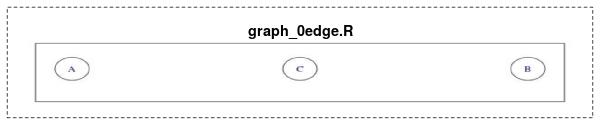
\includegraphics{graph_0edge.jpg} 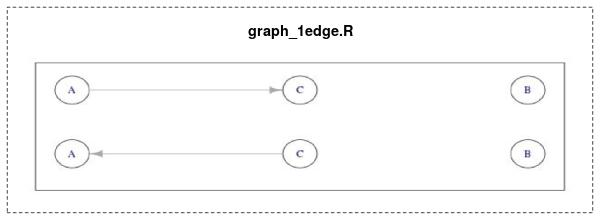
\includegraphics{graph_1edge.jpg}

\begin{figure}
\centering
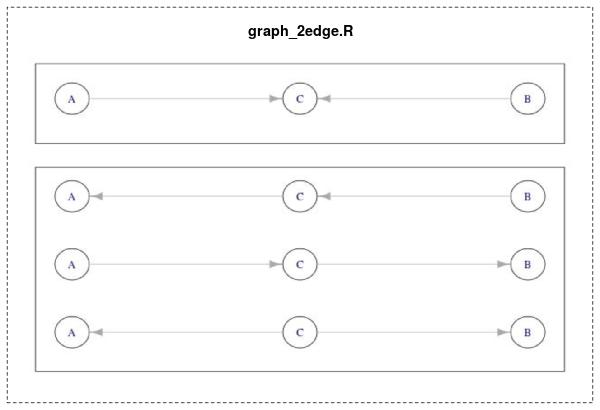
\includegraphics[height=0.50000\textwidth]{graph_2edge.jpg}
\caption{Graph with two edges but not A-B}
\end{figure}

\begin{figure}
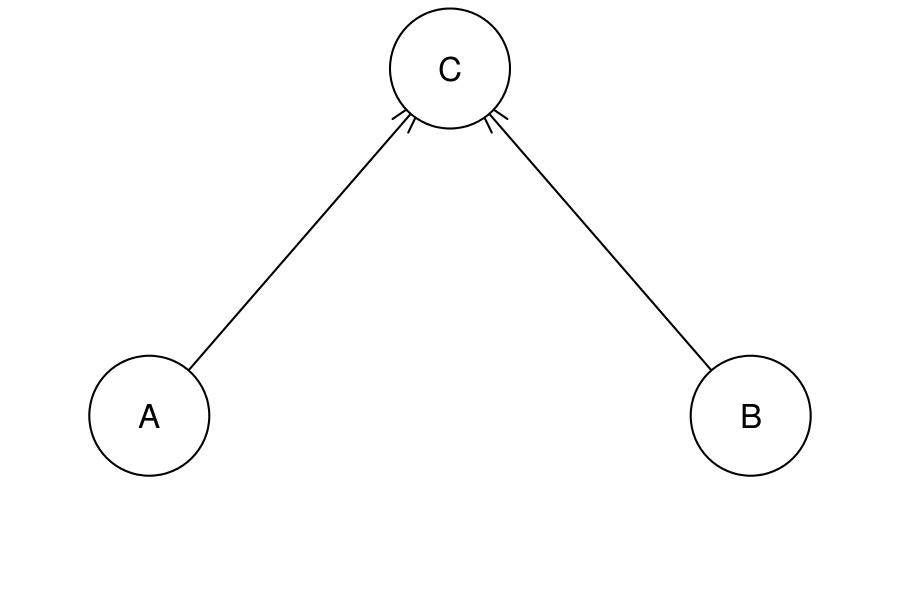
\includegraphics[width=0.45\textwidth]{pcalgo_dat1.png}
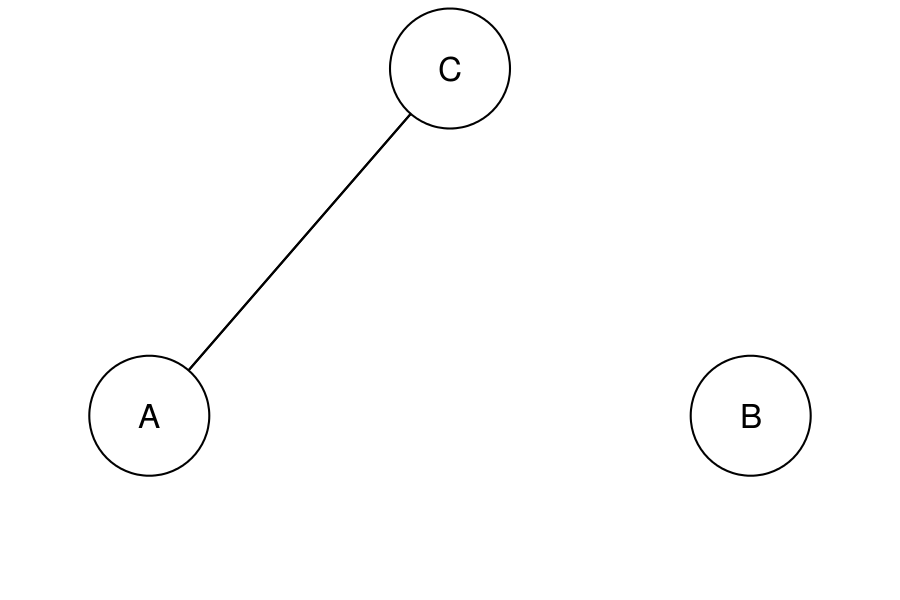
\includegraphics[width=0.45\textwidth]{pcalgo_dat2.png}
\caption{ \label{fig:pc-best}Best networks inferred using "bnlearn::pc.stable". Left: Dataset1. Right: Dataset2}
\end{figure}

\iffalse
\includegraphics[page=1,width=\paperwidth]{popgen_eqn_p3.pdf} \fi

\subsubsection{Comment on the likelihood-equivalent
prior}\label{comment-on-the-likelihood-equivalent-prior}

The likelihood-equivalent prior is set so that the imaginary sample size
decreases as data is stratified by more variables. For example, if
\(P(A=1) \sim Beta(\eta(A_0),\eta(A_1))\), then the imaginary sample
size for (A=1) is \(\eta(A_1)=2\). Hence if we then ask for
\(P(B=1\gvn A=1)\sim Beta(\eta(B_0A_1),\eta(B_1A_1))\), the imaginary
\(\eta\)'s must add up to the imageinary sample size of the condition
\(\gvn A=1\), (aka \(\eta(B_0A_1)+\eta(B_1A_1)=\eta(A_1)=2\)). Assuming
two events are equally probable gives \(\eta(B_0A_1)=\eta(B_1A_1)=1\).
For 3 variable, we can deduce \(8\eta(ABC)=4\eta(AB)=2\eta(A)=\eta(0)\),
setting \(\eta(ABC)=1\) gives
\(\eta(ABC)=1,\eta(AB)=2,\eta(A)=4,\eta(0)=8\), corresponding to
different levels of stratification.

If a likelihood-preserving prior is used, then it is only the
correlation structure that determines the relative feasibility of
different graphs. Consider the 1-edge and 0-edge examples, the 0-edge
example asserts \(P(A\gvn C=0)=P(A\gvn C=1)=P(A)\), whereas the 1-edge
example implies \(P(A\gvn C=0)\neq P(A\gvn C=1)\), allowing an
additional degree of freedom. The striking fact is that this additional
DOF does not necessarily leads to a better model, in constrast to
conventional mixture models where additional components always reduce
likelihood. One of the reason is that the partiaion of
\((A_0)=(A_0C_0)+(A_0C_1)\) is not arbitratry, but the general case is
still confusing. A possible intution is that the additional DOF project
the paramteric space to a higher dimension where the likelihood function
overlaps less with the prior distribution.

\subsubsection{Drawbacks of binary bayesian
networks}\label{drawbacks-of-binary-bayesian-networks}

If there are hidden latent variables in the bayes net, for example where
the common parent of A and B (which is C) is conceived from the
observers, then one will have to consider a graph with hidden variable
in order to explain the data. In other words, a graphical prior needs to
accommodate additional nodes to explain such data. Even though this is
the case, it will be hard to express the case where n(A\_0)=n(B\_0)

\subsubsection{Effect of imaginary sample
size}\label{effect-of-imaginary-sample-size}

Here we consider two imaginary sample sizes \(\eta(0)=8\) and
\(\eta(0)=1\). A higher \(\eta\) indicates a sharper distribution of
binomial probability \(\theta\) (Setting \(\eta(0)=1\) implies
\(\eta(ABC)=0.125,\eta(AB)=0.25,\eta(A)=0.5,\eta(0)=1\))

The corresponding likelihood are calculated for both datasets (dat1 and
dat2, see table \ref{tab:likelihood}).

\begin{itemize}
\item
  For dat1, the chain network (A-B-C) is the best at ISS=1, the A-B..C
  network is the best at ISS=8.
\item
  For dat2, the chain network (A-B-C) is the best for ISS=1 and ISS=8
\end{itemize}

The prediction made by pc.stable is somewhat different (figure
\ref{fig:pc-best})

\begin{figure}
\centering
\includegraphics{net_3var_files/figure-latex/c-gvn-a-idep-1.pdf}
\caption{\label{fig:c-gvn-a-idep}P(C\textbar{}A)=P(C) according to the
0-edge graph, Left: P(C\textbar{}A=0). Right: P(C\textbar{}A=1)}
\end{figure}

\begin{figure}
\centering
\includegraphics{net_3var_files/figure-latex/c-gvn-a-1.pdf}
\caption{\label{fig:c-gvn-a}P(C\textbar{}A) needs to be stratified according
to the 1-edge graph, Left: P(C\textbar{}A=0). Right: P(C\textbar{}A=1)}
\end{figure}

\subsubsection{Plot posteiror for P(C\textbar{}A) in different
models}\label{plot-posteiror-for-pca-in-different-models}

Here I visulise the posterior distribution using dataset 1 only. In
order to show how different graphical models lead to different
likelihood, I chose to contrast P(C\textbar{}A) between
\text{[A][B][C]}(0-edge model) and \text{[A][B][C|A]} (1-edge model)

In 0-edge model, \(P(C|A)=P(C)\) and the distribution is indifferent for
\(A=0\) and \(A=1\) (figure \ref{fig:c-gvn-a-idep}). The term enters
likelihood function as a beta-binomial.

In contrast, the 1-edge model prescribes that \(P(A,C)\neq P(A)P(C)\),
and two separate distribution must be considered for \(P(C|A)\) (figure
\ref{fig:c-gvn-a}). The \(\prod_{C,A} P(C|A)\) term factors out to be
\(\prod_{C|A=0} P(C|A=0)\prod_{C|A=0} P(C|A=1)\), as the product of two
beta-binomial with independent probability but the same prior. It would
be interesting to explore the precise condition under which the factored
likelihood exceeds the original single beta-binomial. Clearly, the
0-edge model fails to capture the difference between \(P(C|A=0)\) and
\(P(C|A=1)\) (loglik=-194.3, compared to 1-edge loglik=-175.5), but the
underlying mathematics remains to be dissected.

\begin{table}

\caption{\label{tab:likelihood}Marginalised likelihood of different network topology}
\centering
\begin{tabular}[t]{l|r|r|r|r|l}
\hline
model & myalgo.bde.iss & bnlearn.bde.iss & bnlearn.bic & iss & dat\\
\hline
[A][B][C] & -194.323 & -194.323 & -195.931 & 8 & dat1\\
\hline
[A][B][C|A] & -175.536 & -175.536 & -176.906 & 8 & dat1\\
\hline
[B][C][A|C] & -175.536 & -175.536 & -176.906 & 8 & dat1\\
\hline
[B][C|B][A|C] & -168.817 & -168.817 & -170.591 & 8 & dat1\\
\hline
[A][C|A][B|C] & -168.817 & -168.817 & -170.591 & 8 & dat1\\
\hline
[C][A|C][B|C] & -168.817 & -168.817 & -170.591 & 8 & dat1\\
\hline
[A][B][C|A:B] & -168.819 & -168.819 & -170.894 & 8 & dat1\\
\hline
[A][B][C] & -196.617 & -196.617 & -195.931 & 1 & dat1\\
\hline
[A][B][C|A] & -177.715 & -177.715 & -176.906 & 1 & dat1\\
\hline
[B][C][A|C] & -177.715 & -177.715 & -176.906 & 1 & dat1\\
\hline
[B][C|B][A|C] & -171.742 & -171.742 & -170.591 & 1 & dat1\\
\hline
[A][C|A][B|C] & -171.742 & -171.742 & -170.591 & 1 & dat1\\
\hline
[C][A|C][B|C] & -171.742 & -171.742 & -170.591 & 1 & dat1\\
\hline
[A][B][C|A:B] & -170.894 & -170.894 & -170.894 & 1 & dat1\\
\hline
[A][B][C] & -195.699 & -195.699 & -197.408 & 8 & dat2\\
\hline
[A][B][C|A] & -180.318 & -180.318 & -181.025 & 8 & dat2\\
\hline
[B][C][A|C] & -180.318 & -180.318 & -181.025 & 8 & dat2\\
\hline
[B][C|B][A|C] & -178.579 & -178.579 & -179.994 & 8 & dat2\\
\hline
[A][C|A][B|C] & -178.579 & -178.579 & -179.994 & 8 & dat2\\
\hline
[C][A|C][B|C] & -178.579 & -178.579 & -179.994 & 8 & dat2\\
\hline
[A][B][C|A:B] & -180.568 & -180.568 & -183.104 & 8 & dat2\\
\hline
[A][B][C] & -198.093 & -198.093 & -197.408 & 1 & dat2\\
\hline
[A][B][C|A] & -181.803 & -181.803 & -181.025 & 1 & dat2\\
\hline
[B][C][A|C] & -181.803 & -181.803 & -181.025 & 1 & dat2\\
\hline
[B][C|B][A|C] & -181.165 & -181.165 & -179.994 & 1 & dat2\\
\hline
[A][C|A][B|C] & -181.165 & -181.165 & -179.994 & 1 & dat2\\
\hline
[C][A|C][B|C] & -181.165 & -181.165 & -179.994 & 1 & dat2\\
\hline
[A][B][C|A:B] & -183.684 & -183.684 & -183.104 & 1 & dat2\\
\hline
\end{tabular}
\end{table}


\end{document}
